\chapter{資料集簡介}
接下來的章節會介紹本論文實驗的過程中,所使用到的音樂資料集,其中除了有網路上對於教學公開的資料集,也有台大MIRLAB實驗室合作對象所提供的資料集,這些資料都極其寶貴,謝謝這些人的付出,對人工智慧在音樂分析領域中做出了極大的貢獻。公開的資料集包含:MUSDB18~\cite{rafii2017musdb18,musdb18}、DSD100~\cite{SiSEC16}、MedleyDB~\cite{bittner2014medleydb}、iKala~\cite{chan2015vocal};非公開的資料集包含:Ke(捷奏錄音室-柯老師)、其餘資料(台大MIRLAB蒐集而成)。接下來會細述這些資料的取得方法,與其內容音檔概述,若要知道粗略的比較可從表\ref{dataset_bref}中取得資訊。另外本章也會概述模型評估基準 Museval~\cite{stoter20182018},其已被打包成 Python 套件方便人工智慧的發展。

\begin{table}[h!]
\centering
\resizebox{\linewidth}{!}{
\begin{tabular}{|r|c|c|c|c|c|c|}
\hline
 & iKala & DSD100 & MedleyDB & MUSDB18 & Ke & 獨立蒐集 \\ \hline
提出年份(公開) & 2015 & 2015 & 2014 & 2017 & N/A & N/A \\ \hline
歌曲資料數 & 306 & 100 & 122 & 150 & 727 & 413 \\ \hline
歌曲時長 & 30秒 & 251±60秒 & 206±121秒 & 236±95秒 & 3~4分鐘 & 3~4分鐘 \\ \hline
總時間長度 & 2小時 & 7小時 & 7.2小時 & 10小時 & 54小時 & 29小時 \\ \hline
完整歌曲/立體聲 & 否/無 & 是/有 & 是/有 & 是/有 & 是/有 & 是/有 \\ \hline
有人聲的歌曲比例 & 100% & 100% & 57% & 100% & 100% & 100% \\ \hline
歌曲分軌數 & 2 & 4 & 1~26 & 4 & 6 & 4 \\ \hline
樂器種類數 & 2 & 4 & 82 & 4 & 6 & 4 \\ \hline
\end{tabular}
}
\caption{資料集概述}
\label{dataset_bref}
\end{table}

\section{MusDB18}
MUSDB18資料集~\cite{rafii2017musdb18,musdb18}\footnote{\url{https://sigsep.github.io/datasets/musdb.html}}由150首不同曲風的雙聲道歌曲組成,其聲音以 44.1khz 編碼,總時長約10小時,聲音分離比賽 2018 Signal Separation Evaluation Campaign~\cite{stoter20182018} 以此資料集為基礎進行,每首歌除了有混音軌(mixture stem),皆包含四個分部:主唱(vocals stem)、鼓 (drums stem)、貝斯(bass stem)、其他(other stem)等4軌。資料集已由官方分成訓練資料和測試資料兩類,其訓練資料共100首,測試資料共50首。資料的來源包含: DSD100 的100首、 MedleyDB 的46首、 Native Instruments 的2首、加拿大樂隊 The Easton Ellises\footnote{\url{https://g.co/kgs/Gqm6Vg}} 的2首。

\subsection{DSD100}
DSD100資料集~\cite{SiSEC16}\footnote{\url{https://sigsep.github.io/datasets/dsd100.html}}由100首不同曲風的雙聲道歌曲組成,聲音分離比賽 Signal Separation Evaluation Challenge 2016~\cite{liutkus20172016} 以此資料集為基礎進行,每首歌除了有混音軌(mixture stem),皆包含四個分部:主唱(vocals stem)、鼓 (drums stem)、貝斯(bass stem)、其他(other stem)等4軌。資料集已由官方分成訓練資料和測試資料兩類,其訓練資料共50首,測試資料共50首。資料的來源是從「'Mixing Secrets' Free Multitrack Download Library」\footnote{\url{https://www.cambridge-mt.com/ms/mtk/}}中汲取而成,特別感謝Mike Senior的允許使用也感謝他對此資料的維護。

\subsection{MedleyDB}
MedleyDB資料集~\cite{bittner2014medleydb}\footnote{\url{https://medleydb.weebly.com/}}由紐約大學音樂與音頻研究實驗室~\footnote{\url{https://steinhardt.nyu.edu/marl}}主導建立,共有196首(44.1kHz、16bit)的歌曲,資料集詳細註記每首歌曲的資訊:曲風、歌曲長度、作曲者、歌手性別等等,對每首歌曲以樂器為單位詳細記錄其分軌,一首歌曲可能會被分成數10軌不等,有助於研究不同歌曲造成差異的原因。圖 \ref{medleyDB_inst}和圖 \ref{medleyDB_genre} 為音軌和曲風的詳細資訊。

\begin{figure}[htbp]
    \centering
    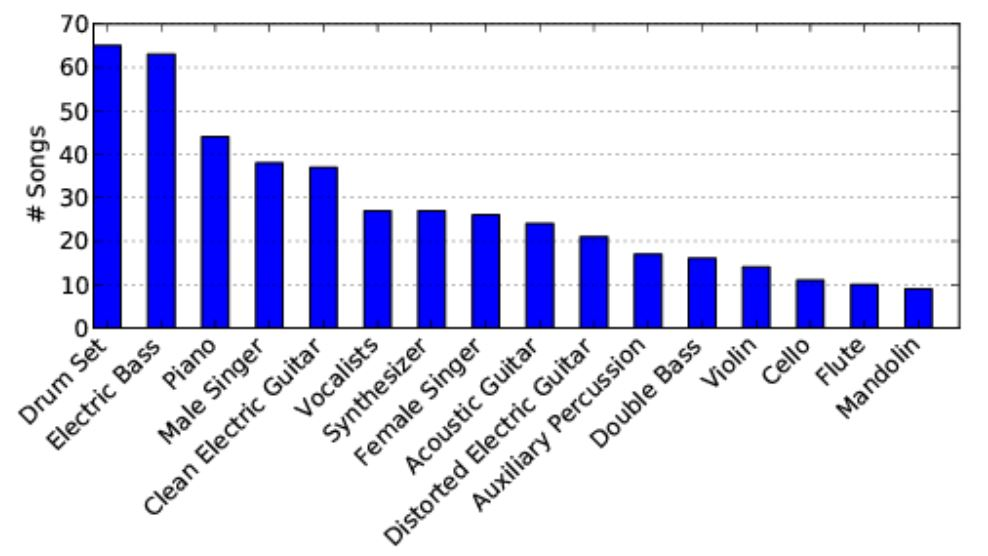
\includegraphics[width=0.6\textwidth]{./figures/chapter03_dataset/medleyDB_inst.jpg}
    \caption{MedleyDB音軌資訊}
    \label{medleyDB_inst}
\end{figure}
\begin{figure}[htbp]
    \centering
    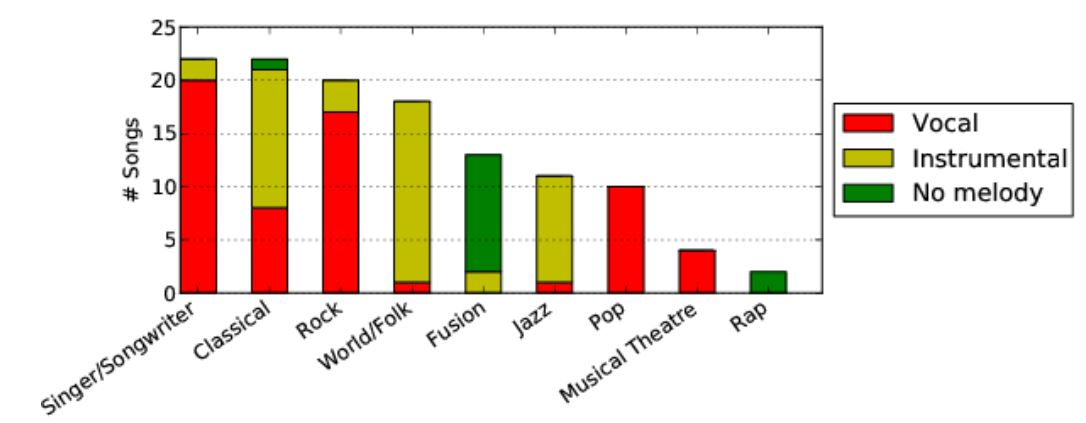
\includegraphics[width=0.8\textwidth]{./figures/chapter03_dataset/medleyDB_genre.jpg}
    \caption{MedleyDB曲風資訊}
    \label{medleyDB_genre}
\end{figure}

\subsection{Museval 模型測試指標}
% stoter2018museval,stoter20182018
在提及此測試指標之前,需先提到一個音樂分離比賽,也就是 2018 Signal Separation Evaluation Campaign~\cite{stoter20182018},其比賽除了透過MUSDB18資料集~\cite{rafii2017musdb18,musdb18}進行,另外提供了一個Python套件\footnote{\url{https://github.com/sigsep/sigsep-mus-eval}}稱為Museval~\cite{stoter2018museval},方便指標的計算與模型評估。此指標被多數音樂分離領域的研究中採用,其中有兩大開源實驗項目:Facebook 開發的 Demucs\footnote{\url{https://github.com/facebookresearch/demucs}} 、Deezer 開發的 Spleeter\footnote{\url{https://github.com/deezer/spleeter}},皆使用此評估開發中的模型優劣,目前可見的論文也都採用此,這極大地幫助實驗進行。套件目的在於評估分離模型分析的結果並輸出有效的 json 檔案,希望研究人員使用此評估輸出格式作為「共享分離結果」的標準,Museval 設計與 Musdb18 結合使用。


\section{iKala}
iKala資料集~\cite{chan2015vocal}\footnote{\url{http://mac.citi.sinica.edu.tw/ikala/}}是在MIR-1K資料集之後,由iKala、台大 MIRLAB 和中研院 MACLAB\footnote{\url{http://mac.citi.sinica.edu.tw/}} 共同建立的高品質分軌歌曲資料集,並且也是為數不多的中文歌曲資料集,其中資料是從206首歌曲中以30秒為單位並用44.1kHz進行採樣,最後取得252個片段,且每個片段都已經分軌為人聲和背景音樂資料,此外,iKala中的每首歌曲都有標記音高和歌詞出現的時間點,讓可以使用此資料集的研究領域更廣,表\ref{comp_mir_1k_with_ikala}為 MIR-1K 與 iKala 資料集的比較。

\begin{table}[h!]
\centering
\begin{tabular}{|r|c|c|}
\hline
\textbf{}                 & \textbf{MIR-1K} & \textbf{iKala} \\ \hline
Sample rate               & 16kHz           & 44.1kHz        \\ \hline
Singer quality            & Amateur         & Professional   \\ \hline
Clip duration             & 4-13s           & 30s            \\ \hline
Number of clips           & 1000            & 252            \\ \hline
Voice recorded separately & Yes             & Yes            \\ \hline
Pitch contour annotations & Yes             & Yes            \\ \hline
Voice type annotations    & Yes             & No             \\ \hline
Lyrics with speech        & Yes             & No             \\ \hline
Lyrics with timestamps    & No              & Yes            \\ \hline
Separate chorus and verse & No              & Yes            \\ \hline
Instrumental solo         & No              & Yes            \\ \hline
\end{tabular}
\caption{MIR-1K與iKala資料集的比較}
\label{comp_mir_1k_with_ikala}
\end{table}

\section{捷奏錄音室-柯老師}
資料集由本次研究合作的捷奏錄音室提供,捷奏錄音室是民國78年創立時,國內少數專業的大型錄音室。在此資料集中,總共有727首分軌歌曲,MIRLAB將歌曲資料經過處理後,最後依照一般歌曲的主要樂器分成6軌,分別為:主唱(vocals stem)、鼓 (drums stem)、貝斯(bass stem)、其他(other stem)、吉他(guitar stem)、電吉他(e-guitar stem)。此資料集的歌曲包含許多中文流行音樂、鄉村音樂,大量的歌曲資料有助於增加機器學習模型訓練效果。

\section{其餘資料收集}
MIRLAB的黃翔宇~\footnote{hsiangyu.huang@mirlab.org}透過目前現有的歌曲分離來源技術,對混音好地近年熱門流行歌曲進行分離,因此對應每個音軌並不是完全正確的。總共有413首歌曲,並將每首歌曲都分成4軌,主唱(vocals stem)、鼓 (drums stem)、貝斯(bass stem)、其他(other stem)。